\documentclass[sigconf]{acmart}

\usepackage{graphicx}
\usepackage{algorithm} % for algorithms
\usepackage{algpseudocode}
\usepackage{booktabs} % For formal tables
\usepackage{amsthm} % For claims

\theoremstyle{remark}

\settopmatter{printacmref=false, printccs=true, printfolios=true}
\pagestyle{empty} % removes running headers

\newcommand{\PicScale}{0.5}
\newcommand {\FlameStream} {FlameStream}
\begin{document}

\copyrightyear{2019} 
\acmYear{2019} 
\setcopyright{acmcopyright}
% \acmConference[BeyondMR'18]{Algorithms and Systems for MapReduce and Beyond }{June 15, 2018}{Houston, TX, USA}
% \acmBooktitle{BeyondMR'18: Algorithms and Systems for MapReduce and Beyond , June 15, 2018, Houston, TX, USA}
% \acmPrice{15.00}
% \acmDOI{10.1145/3206333.3209273}
% \acmISBN{978-1-4503-5703-6/18/06}

\title {Distributed Classification of Multi-Labelled Text Streams}

% \author{  Igor E. Kuralenok,$^1$     Artem Trofimov,$^ {1,2}$    Nikita Marshalkin,$^ {1,2}$   and  Boris Novikov$^ {1,2}$ }
% \affiliation{%
% \institution{$^1$JetBrains Research}
%   \city{St. Petersburg} 
%   \country{Russia}
% }
% \affiliation{%
% \institution{$^2$Saint Petersburg State University}
%   \city{St. Petersburg} 
%   \country{Russia}
% }
% \email{\string{ikuralenok, trofimov9artem, marnikitta\string}@gmail.com, borisnov@acm.org}

\begin{abstract}

%Задача классификации текстов является хорошо изученной, однако когда данные являются потоковыми начинаются трудности. При такого рода данных, основная сложность является в обеспечении малой задержки между получением очередного текста и его разметкой. Задача обработки текстов на потоковых данных известна, однако существующие решения либо batch processing либо не являются масштабируемыми, также эти решения не обладают гибкостью к постоянно изменяющимся потоку данных. В нашей работе мы представляем систему, где нам удалось создать решение, обеспечивающее минимальную задержку при классификации текстов, при этом, проходить дообучение в реальном времени, сохраняя эту задержку. Мы провели эксперименты, показывающие успешность наших результатов.

Multi-labelled text classification problem is well-known one, but classifying text data on streams is a challenging task. Due to the nature of data, the main difficulty is providing a low latency between obtaining text and its labeling. There are solutions of processing texts on streams, however, they are either batch based or non-scalable ones, in addition, this techniques do not adopt to constantly evolving data stream. In this work, we introduce a system, which manages the previous aspects and providing low latency, moreover, the system is able to continue training in real-time without compromising the latency. Our experiment results demonstrate the benefits of our approach.

% Комментарии БА: нет постановки задачи из-за этого все едет.
% Как такого request-а нет -- при написании слова реквест кажется, что как будто пользователь его делает, но это не так.
% Prior research on processing streaming data has been worked only on batch based solutions or non-scalable ones. However, due to the nature of data is critical to have a scalable solution, moreover, obtaining an answer for a [request] essentially to have low latency. In this paper, we propose text classification on streaming data, where this aspects were considered. Our system is able to continue to fit on the fly without compromising the latency, but increasing answer accuracy instead.

\end {abstract}

% \keywords{Data streams, exactly-once, drifting state, optimistic OOP}

\maketitle

\thispagestyle{empty}

\section {Introduction}
\label {fs-short-intro}

Classification of large text streams is hard, but important task for researchers and practitioners. It has a wide range of applications including detection of emerging news and current user interests, suspicious traffic analysis, spam filtering, etc. Popular open-source libraries like sklearn~\cite{sklearn_api} and NLTK~\cite{bird2009natural} provide a rich set of tools, but they mostly aim at handling static datasets. The lack of scalability across multiple computational units is another limitation of these solutions. There are plenty of works which adapt batch processing systems for text classification~\cite{semberecki2016distributed, svyatkovskiy2016large, baltas2016apache}. Their advantages are fault tolerance, high throughput, and scalability. On the other hand, these systems do not provide low latency that is a strong requirement for most streaming applications.

An immediate idea is to employ a distributed stream processing engine such as Flink~\cite{Carbone:2017:SMA:3137765.3137777} or Storm~\cite{apache:storm}. However, stream processing systems have several important differences in comparison with batch engines: 

\begin{itemize}
    \item In a general case, failure and recovery are not transparent for a user. The guarantees on data in case of failures are defined in terms of delivery guarantees: {\em at least once} and {\em exactly once}. The choice of a guarantee may affect the correctness of text classification.
    \item Most of streaming systems are inherently non-deterministic. It means that different runs on the same data may produce different results. This feature can influence the classification process as well.
\end{itemize}

In this work, we investigate the applicability of state-of-the-art stream processing systems to the text classification and demonstrate the challenges that a developer can experience. Our study reveals issues similar to the problems mentioned by TFX project team~\cite{Baylor:2017:TTP:3097983.3098021} on machine learning at scale in general: reproducibility, reliability of results, fault tolerance, etc. For demonstration, we adapt text classification data flow that is typical for batch processing systems for state-of-the-art stream processing engine Apache Flink~\cite{Carbone:2017:SMA:3137765.3137777}. We show that failures within {\em at least once} guarantee may significantly shift the distribution of classification results. It is also indicated that races due to asynchronous channels in the data flow lead to a non-reproducible outcome. We demonstrate that straightforward solutions to the revealed issues may lead to performance overhead. More sophisticated approaches to solve the problems are touched upon.

The rest of the paper is structured as follows: the problem of text classification using stream processing engines and the typical data flow are discussed in section~\ref{fs-framework}, section~\ref{fs-discussion} contains the evaluation of the data flow on top of state-of-the-art stream processing system, approaches to get around the revealed issues are introduced in section~\ref{fs-solution}, prior works on the topic are mentioned in section~\ref{fs-related}, we discuss the results and our plans in~\ref{fs-conclusion}.

\section {Experiments}
\label {fs-experiments}

To prove the feasibility of the proposed framework we conducted a series of experiments. We show the efficiency and scalability of the distributed streaming dataflow on the top of~\FlameStream\ processing system. Latency and throughput are used as performance metrics. We also demonstrate achieved accuracy using a simple machine learning model. As a dataset, we used an open corpus of news articles from Russian media resource lenta.ru~\cite{lentaru}. This dataset contains about 700 000 documents, which are labeled by one of 90 different topics. In the experiments, we generated a stream consisted of articles from the dataset sorted by the time of publishing.

\begin{figure}[htbp]
  \centering
  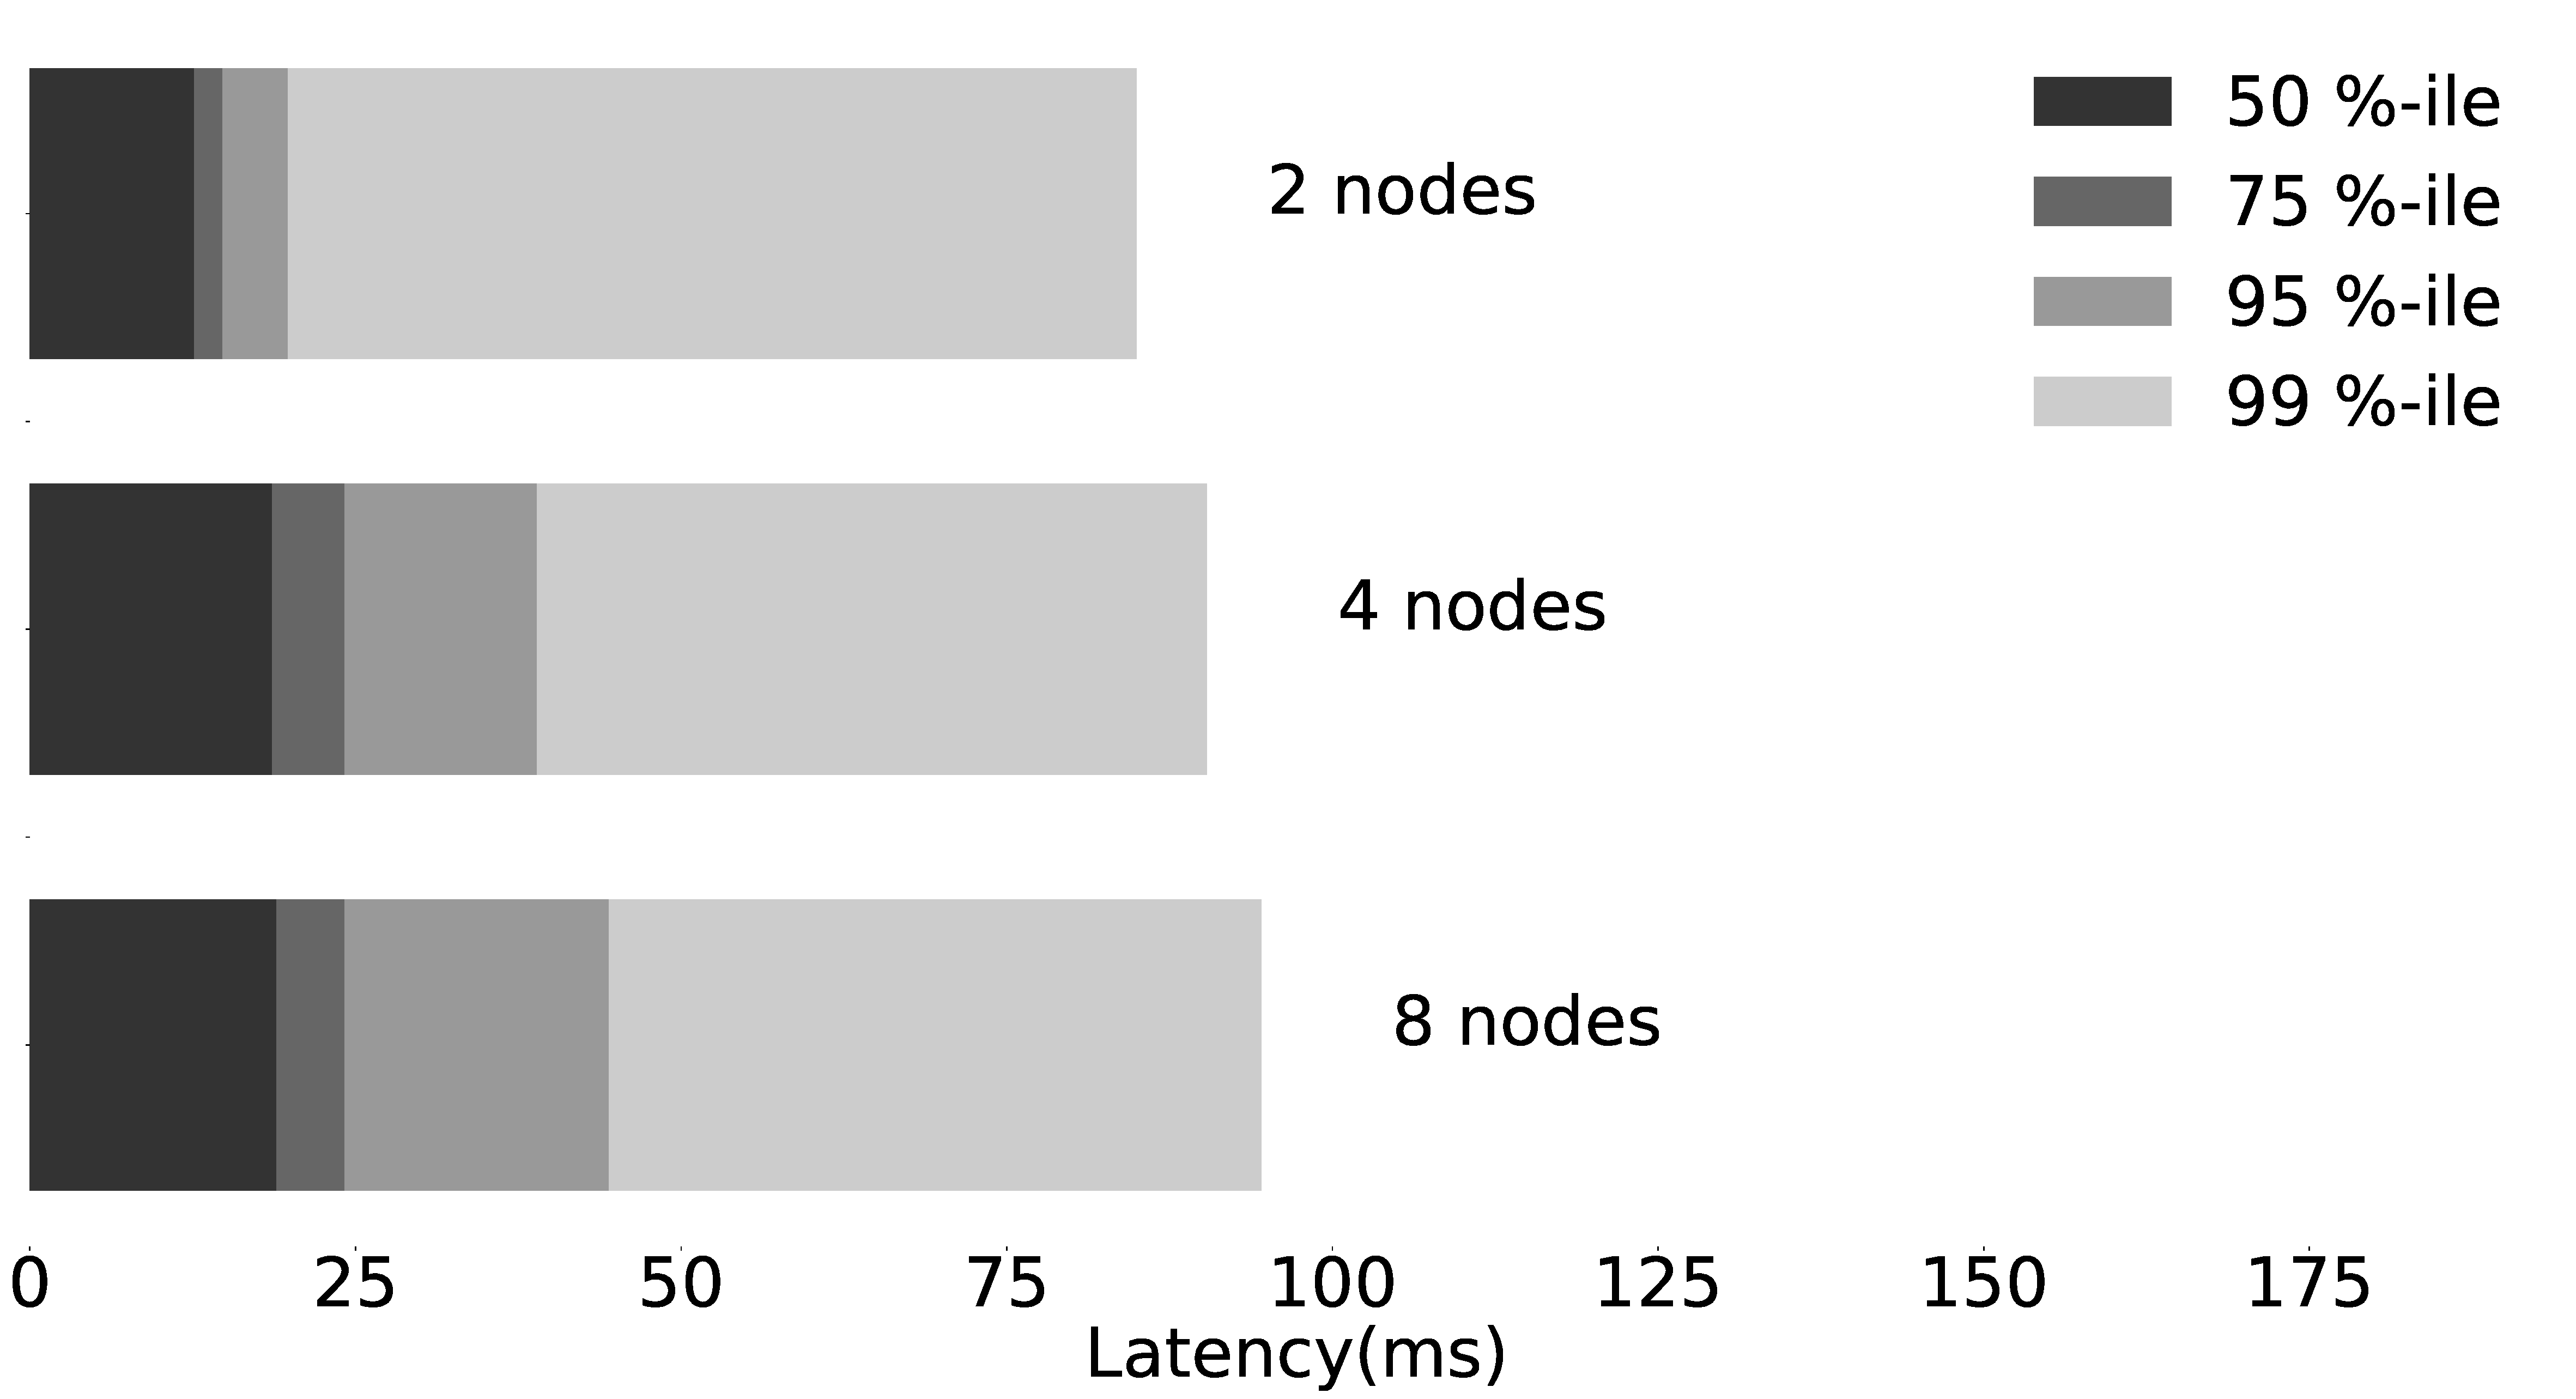
\includegraphics[scale=0.1]{pics/classifier_latencies}
  \caption{Prediction pipeline latencies}
  \label {latencies}
\end{figure}

\subsection{Data flow evaluation}

For evaluation, we deployed FlameStream on clusters, containing 2, 4 and 8 Amazon EC2 small instances with 2 GB of RAM and 1 core CPU. Exactly once guarantee was enabled. We measured throughput that is possible to achieve and the corresponding latency for prediction pipeline\footnote{We took into consideration only the performance of the streaming pipeline without a persistent queue}. The results are shown in Figures~\ref{latencies} and~\ref{throughput}. As we can see, there is a linear trend in throughput, which proves the scalability of the framework. On the other hand, one can observe, that latency increases moderately and keeps under 25 ms for a median and under 100 ms for 99th percentile.

\begin{figure}[htbp]
  \centering
  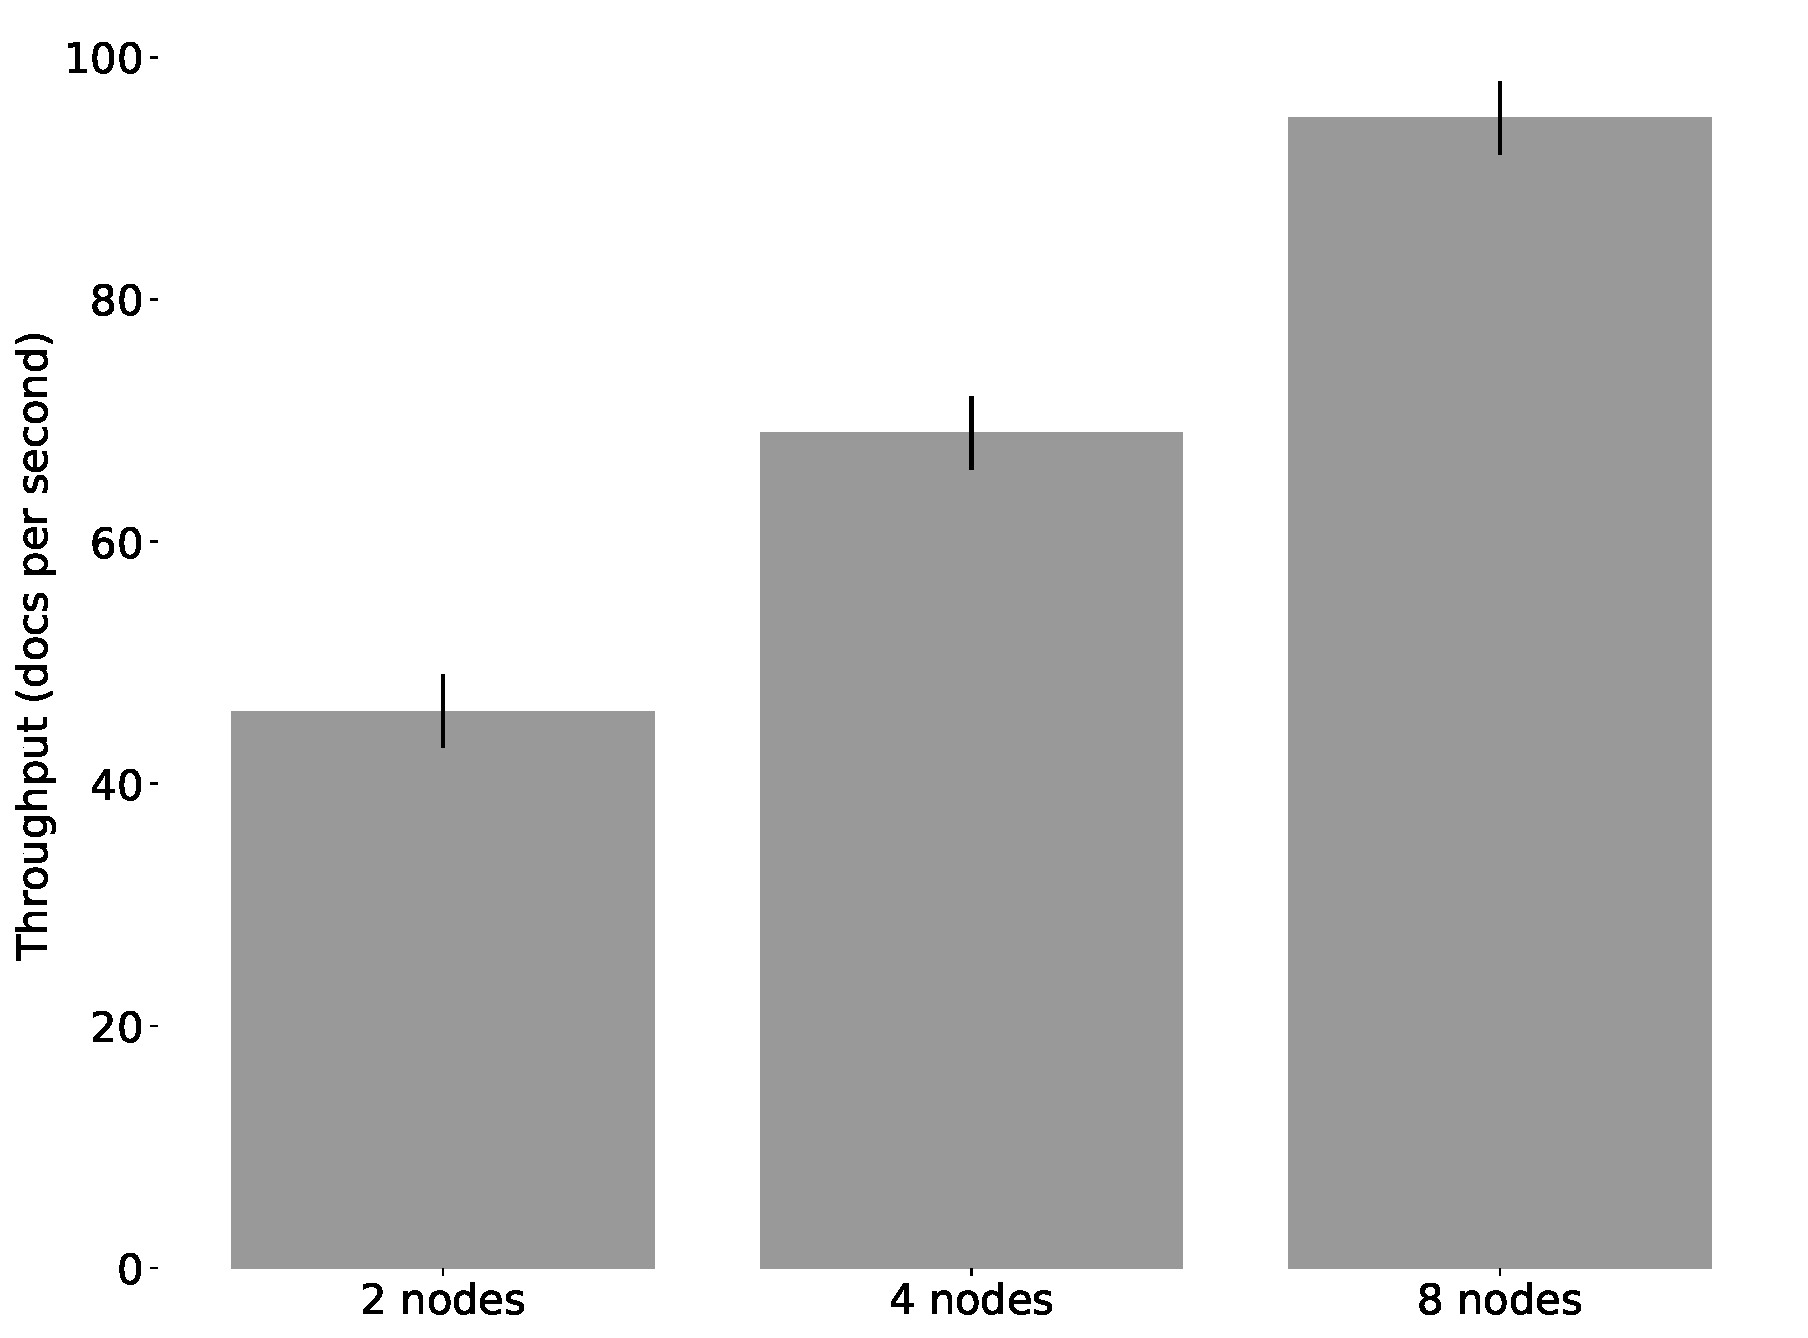
\includegraphics[scale=0.21]{pics/classifier_throughput}
  \caption{Prediction pipeline throughput}
  \label {throughput}
\end{figure}

\subsection{Classifier evaluation}

In order to be efficiently embedded in the proposed data flow, several properties of the machine learning model are desirable:
\begin{itemize}
     \item Small size of the model for storing and updating it in reasonable time and space.
     \item A possibility to update the model with new data.
\end{itemize}

We use Multinomial Logistic Regression as a classification method. Model parameters (weights) are denoted as $W$. The training process is the maximization of the following formula in terms of $W$:

$$ 
\begin{array}{rcl}
\log P(W | X)   & = &
 \frac 
      {1}{|X|} \sum \limits_{(x, y) \in X} \log \frac{e^{{W_y^T \cdot \; x}}}
      {\sum \limits_{l = 1}^{k}  e^{{W_{l}^T \cdot \; x}}}                  \\
  & & - \lambda_1 \parallel  W\parallel _1 
   - \lambda_2 \parallel  W - W_{prev} \parallel _2 
   \end {array}
   $$ 

$X$ denoted as a training dataset and the number of classes is $k$. Also, $x$ designated as a point in the dataset and $y$ as a label for it. To change the model over time, we use weights that are computed in the previous step -- $W_{prev}$. At the first step, $W_{prev}$ can be provided by a pre-train process.

The first component is the standard softmax function for multiple classes. The second component keeps the $L1$ regularization of the weights, and provides sparsity: with the dictionary of size 560 000, there is only 2\% of non-zero elements in $W$. Hence, the model has a small size -- about 10 Mb. We apply $L2$ regularization as the third component in order to use previous weights for on-the-fly model update.

We compared two approaches to the performance evaluation of the proposed machine learning model. The first one is training on the complete dataset with $\lambda_2 = 0$. We call this approach a {\em static training}. The second one consists in dividing training dataset into relatively small batches and consequent applying MLR with $L2$ regularization to each batch. The latter case demonstrates the behavior of our streaming classification approach. Dividing into train and test samples must be done uniformly in time in order to fairly evaluate streaming classifier. We calculate a hash function that depends on an input text to determine the use of text either in training or in the test sample. The sizes of the train and test sets are 50 000 and 100 000. The size of batches for the streaming approach is 5 000.

As one can see in Table~\ref{accuracy}, the streaming approach has a slightly lower accuracy in comparison with the static. The achieved value is reasonable considering the number of classes. These results indicate that our framework is able to efficiently solve the text multi-classification problem.

\begin{table}[htbp]
\caption{Accuracy comparison between static and stream training}
\begin{tabular}{lc}
Method             & Accuracy \% \\
Static training    & 0.609       \\
Streaming training & 0.601         
\end{tabular}
\label{accuracy}
\vspace{-7mm}
\end{table}

\section {Conclusion}
\label {fs-conclusion}

In this work, we investigated the suitability of distributed stream processing engines to the problem of text streams classification. We demonstrated that there are several pitfalls with an adaptation of data flow commonly used in batch systems for a stream processing:

\begin{itemize}
    \item Races in a physical data flow lead to irreproducible results: labels provided by a classifier may vary from run to run on the same test data. 
    \item Failures within {\em at least once} delivery guarantee can cause a biased distribution of classification results.
    \item Streaming data is rapidly changing, so there is a need to update the machine learning model on-the-fly. 
\end{itemize}

It was shown that straightforward solutions to the mentioned issues imply significant performance overhead. There were proposed potential solutions: to use~\FlameStream\ processing system with built-in determinism and efficient exactly once and to embed online learning into the data flow. 

As future work, we plan to implement a text classification framework that satisfies the following requirements:

\begin{itemize}
    \item Unbiased by distributed environment: node failures or races do not affect the ultimate result distribution.
    \item Reproducible: if input elements are stored in persistent storage, the same predictions are obtained on each new run.
    \item Concept drift conscious: changes in streaming data must be reflected in a machine learning model.  
\end{itemize}

\bibliographystyle{ACM-Reference-Format}
\bibliography{../../bibliography/flame-stream}

\end {document}

\endinput
